The architecture was built through the iterative methodology called AOPOA and the starting point was the global agent's goal of perform a sequence of actions coherent with a given script. The AOPOA methodology allow the decomposition of goals in smaller goals until the desired granularity is reached. This section describes the final result of this methodology showing in the \ref{fig:generalArchitecture} In this view its shown the structural composition of an robo-actor as a subset of functional components, each component belongs to a group that encapsulate a specific internal process.
\begin{figure}
	\centering
	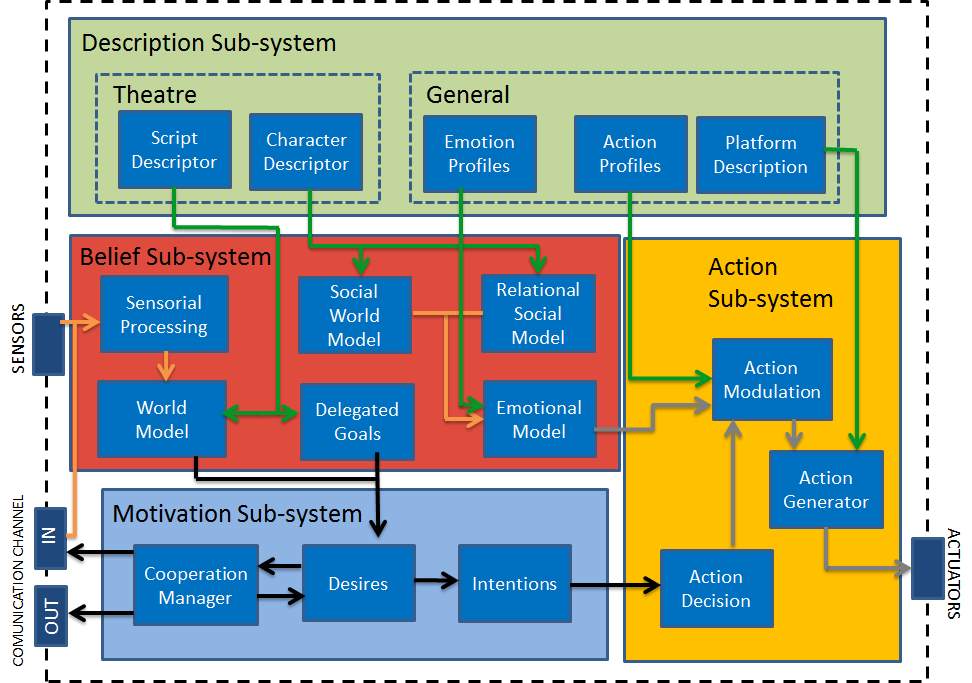
\includegraphics[width=0.5\textwidth]{Images/GeneralArchitecture.png} 
	\caption{General architecture . The green arrows show the information that comes from the configuration module about the script information and the robotic platform information. The orange arrows are information that is relevant to update the beliefs and the internal state of the agent. The black arrows represent information about the current goals that the agent wants to achieve and how this information becomes in an action. Finally, the gray arrow represent how the action is affected by the emotional state and how the action is executed in the current platform's agent.}
	\label{fig:generalArchitecture}
\end{figure}


\subsubsection{Belief Manager}

This group handle the goal of maintain and update the mental state of the robo-actor agent. This goal is achieve in two different ways. First, the perception phase collect and process relevant information about the world and update its internal model of the world. Then, how is handle the emotional state of the robo-actor?. This is achieve through the script provided by the configuration module. It means, the emotional state and the belief about its social environment only occurred inside the play and its governed by the script definition.

\subsubsection{Motivation Manager}

The motivation manager is in charge of the deliberative process, in other words  this group is responsible for the big question: what should the agent do?. The design of this group has done in concordance with the belief-desired-intention model but also, incorporate a communication manager that allow the coordination between robo-actors when it is required.

\subsubsection{Action Controller}

The action define in the deliberative process remains incomplete for the purpose of architecture. It is because of the lack of emotional intervention in the decision making process. Then, the action controller makes the modulation of the action according to the emotional state of the agent. In this way the emotional state does not interfere in the decision process, crucial for the theatrical performance, instead add naturalness and emotion that traduces in a better perception of the agent performance. The final phase is the translation of the action in terms that the specific platform can understand and execute, this process is supported in the platform descriptor provided by the configuration module of the agent.